\documentclass[11pt, a4paper]{article}
\usepackage{tikz}
\usepackage{circuitikz}
\usepackage{float}
\usepackage{amsmath}
\usepackage{graphicx,epsfig}
\usepackage{verbatim}
\usepackage{enumerate}
\usepackage[margin=.8in]{geometry}
\providecommand{\e}[1]{\ensuremath{\times 10^{#1}}}

\title{MEng Thesis \\ Circuit Sensing Breadboard}
\author{Josh Gordonson}

\begin{document}
\maketitle

\section{Motivation}
The breadboard has been a staple substrate for electronic construction over the last century.
At the dawn of a growing interest in amatuer radio, resourceful tinkerers used planks of wood to secure and ruggedize their electrical handiwork.
%Breadboarding was a construction technique that enabled reconfigurable experiments or permanent electrical machines
%---------------------------------BREADBOARD FIGURE-------------------------------
Conductive nodes, such as nails or copper rails, were driven into the non-conductive boards, providing anchors and contact points that were electrically isolated from the rest of the circuit.
Components were soldered or wire-wrapped to the nodes, and sometimes secured by non-energized nails or screws.
This construction technique provided a lot of artistic freedom in circuit construction, but was time consuming and required relatively heavy hand tools such as a hammer or drill.

The solderless breadboard is the cannonical tool given to students taking introductory courses in the field.
Rather than driving nodes into arbitrary locations, component leads are inserted into contact points arranged on a grid that allow rapid semi-rigid construction of circuits with no other tools.
%-------------------------------BREADBOARD FIGURE-----------------------------
The layout of a solderless breadboard is designed to be compatible with a plethora of powerful integrated circuits, enabling complex designs.
Modern solderless breadboards have come a long way from their namesake wooden ancestors, but there is still room for improvement.

The shortcomings of solderless breadboards lie entirely within the art of breadboarding.
The intent of breadboarding is to physically realize a circuit.
Often, this involves designing or using a reference schematic to guide construction, but circuit improvisation is not uncommon.
Inserting components and jumper wires into contact points is straightforward, but poor contacts, broken wires (inside insulation), and mis-inserting leads can plague designers for hours on end and potentially destroy components.
A meticulous breadboarder can successfully realize a circuit without error, but for the uninitiated it is difficult to justify the additional time and care required to plan and build.
Breadboarding is a skill that is learned over time, but small errors can lead to excessive frustration and turn students off to the field.
To satisfy the requirements of the Masters in Engineering program, I propose a solution to some of the issues with the solderless breadboard.

\section{Overview}

A confident linkage between the the electrical and mechanical domains is required to construct a circuit.
On larger scales, the mechanical structures (eg. contacts, wires, components) that create electrical circuits are visible in plain sight.
It is simple and reliable, then, to determine the circuit representation of a mechanical structure that has no hidden connections.
Breadboards often obscure connections due to their construction.
The regular nature of a breadboard, a grid of contact points arranged in rails, makes it difficult to keep track of which rail is connected to what circuit node.
When combined with the opaque nature of most components and the poor reliability of breadboard contacts, visually verifying complex circuits on a breadboard becomes infeasible.
Many of the inherent problems with breadboards stem from this open-loop nature of breadboarding, where visual cues are not enough to determine the electrical circuit from the mechanical structure.
A symptom of open-loop construction techniques is a mismatch between the mental model and the physical realization of the system at hand.
I seek to close this loop by designing and implementing a circuit-sensing breadboard.

At first glance, the proposed problem is straightforward.
A standard-issue breadboard has 130 conductive rails.
Each of these rails can be connected to an array of ADCs (analog to digital convert-
ers) and DACs (digital to analog converters) controlled by a microcontroller.
With access to every node in the circuit, it is possible to determine a constructed circuit's topology by iteratively stimulating and probing the circuit.
Further, a schematic representation of the circuit topology can be drawn on an available display.
This visual display provides an accurate depiction of the electrical circuit at hand, effectively closing the loop on breadboard construction.
%---------------------BREADBOARD VS BUTTERBOARD FIGURE-------------------------
Designing a circuit-sensing breadboard requires a substantial amount of hardware and software infrastructure.
Fortunately, the majority of this infrastructure is useful in its own right.

A hardware test-bench was constructed to interface each of the 130 rails on the breadboard.
The test-bench is composed of a pcb-mounted breadboard, an ADC and DAC multiplexing board, a microcontroller, firmware to control sampling and stimulating the breadboard, and software to stream the sampling data to a computer for display.
Effectively, the test-bench is a 130-channel digital breadboard-oscilloscope/function generator.
Since software is faster to prototype with, the theoretical circuit topology work was first implemented in software.
A circuit simulator test-bench was written to provide the circuit-sensing algorithm in development with data.
This test-bench allows the circuit-sensing algorithm to probe, stimulate, and ground every node of a randomly generated circuit, as if the circuit were built on a breadboard attached to the hardware test bench mentioned above.
The software test-bench also had the ability to print out a circuit network solution to a schematic display.

\section{Work to Date}

\subsection{RLC network sensing algorithm}

Electrical impedance is a measure of the complex voltage $\tilde{V}$ across two nodes divided by the complex current $\tilde{I}$ through those nodes.
The magnitude of the impedance is
Circuit elements can be identified by their characteristic impedances.
An ideal resistor has an impedance that resistance.
$Z_R=r$.
An ideal inductor has an impedance that is imaginary and proportional to frequency.
$Z_L=j\omega l$.
An ideal capacitor has an impedance that is inversely proportional to frequency.
$Z_C=\frac{1}{j \omega c}$.
Impedance analyzers are commercial devices that measure the impedance of an element between its terminals.

The impedance network sensing algorithm relies on the ability to probe any node voltage, add a voltage source with a current meter to any node, and ground any node.
In particular, the ability to ground any node in the network significantly reduces the network's complexity, which makes designing an algorithm to determine any branch impedance rather straightforward.
The impedance network sensing algorithm works as follows:
\begin{figure}[h]
  \begin{center}
    \begin{circuitikz}
		\draw (0,0)
		node[label={below:$1$}] {}
		to[R=$Z_{13}$] (1.5,2.584)
		node[label={above:$3$}] {}
		to[R=$Z_{35}$] (3,0) % The resistor
		node[label={below:$5$}] {}
		to[R=$Z_{15}$] (0,0)
		to[R=$Z_{12}$] (-1.5,2.584)
		node[label={above:$2$}] {}
		to[R=$Z_{23}$] (1.5,2.584)
		to[R=$Z_{34}$] (4.5,2.584)
		node[label={above:$4$}] {}
		to[R=$Z_{45}$] (3,0);
		\fill (0,0) circle (1mm);
		\fill (3,0) circle (1mm);
		\fill (1.5,2.584) circle (1mm);
		\fill (4.5,2.584) circle (1mm);
		\fill (-1.5,2.584) circle (1mm);
    \end{circuitikz}
   \caption{Example Circuit}
  \end{center}
\end{figure}
\begin{enumerate}
\item[1] - Pick a circuit branch [$b_1$] between two nodes [$n_1$] and [$n_2$] to identify
\item[2] - Add a voltage source to [$n_1$] and ground every other node in the circuit
\item[3] - Divide the voltage at [$n_1$], [$V_{n_1}$], by the voltage source current [$I_{VS}$] to obtain the parallel impedance of all branches connected to [$n_1$], [$Z_{1_{||}}$]
\item[4] - Add a voltage source to [$n_2$] and ground every node in the circuit except for [$n_1$] and [$n_2$]
\item[5] - Divide [$Z_{1_{||}}$] by the resulting voltage measured, [$V_{n_1}$] to obtain the impedance of [$b_1$], [$Z_{12}$]
\item[6] - Repeat 1-5 for all pairs of nodes in the network
\end{enumerate}
Step [5] is a bit magical, so let's look at a quick example from Figure 1:
First, let's pick nodes $1$ and $3$, apply a voltage source to node $1$ and ground all of the other nodes.  \\
The resulting $\displaystyle Z_{1_{||}} = Z_{13}||(Z_{12}||Z_{15})= \frac{Z_{13}(Z_{12}||Z_{15})}{Z_{13}+(Z_{12}||Z_{15})}$\\
Now, we apply a voltage source to node $3$, open node $1$, and ground all of the other nodes.\\
The voltage that appears at node $1$, $\displaystyle V_{n_1} = \frac{V_{n_3} Z_{12}||Z_{15}}{Z_{13}+Z_{12}||Z_{15}}$\\
Finally, $\displaystyle \frac{Z_{1_{||}}}{V_{n_1}}=\frac{\frac{Z_{13}(Z_{12}||Z_{15})}{Z_{13}+(Z_{12}||Z_{15})}}{\frac{Z_{12}||Z_{15}}{Z_{13}+Z_{12}||Z_{15}}}=Z_{13}$

To determine if there are multiple element types [in parallel] between two nodes, we can select a few frequencies to scan through and analyze the resulting change in impedance.

\begin{figure}[h]
  \begin{center}
    \begin{circuitikz}
		\draw (0,-.5)
		node[label={below:$2$}] {}
		to[short] (0,0)
		to[R=$R$] (0,2)
		to[short] (1.5,2)
		to[L=$L$] (1.5,0) % The resistor
		to[short] (-1.5,0)
		to[C=$C$] (-1.5,2)
		to[short] (0,2)
		to[short] (0,2.5)
		node[label={above:$1$}] {};
	    \fill (0,-.5) circle (1mm);
		\fill (0,2.5) circle (1mm);
    \end{circuitikz}
   \caption{Example RLC Tank Circuit}
  \end{center}
\end{figure}

The impedance of a parallel RLC 'tank' circuit can be characterized and analyzed over all frequencies.

\begin{align}
Z_C = \frac{1}{j\omega C} \qquad Z_R = R \qquad Z_L = j\omega L \\
Z_{RLC}=Z_C||Z_R||Z_L = \frac{1}{j\omega C+\frac{1}{R}+\frac{1}{j\omega L}}= \frac{j\omega RL}{-\omega^2RLC+j\omega L+R}
\end{align}

$\displaystyle Z_{RLC}$ has a zero at $\frac{1}{RL}$ and two poles at $\frac{-L^{+}_{-}\sqrt{L^2+4R^2LC}}{-2RLC}$\\
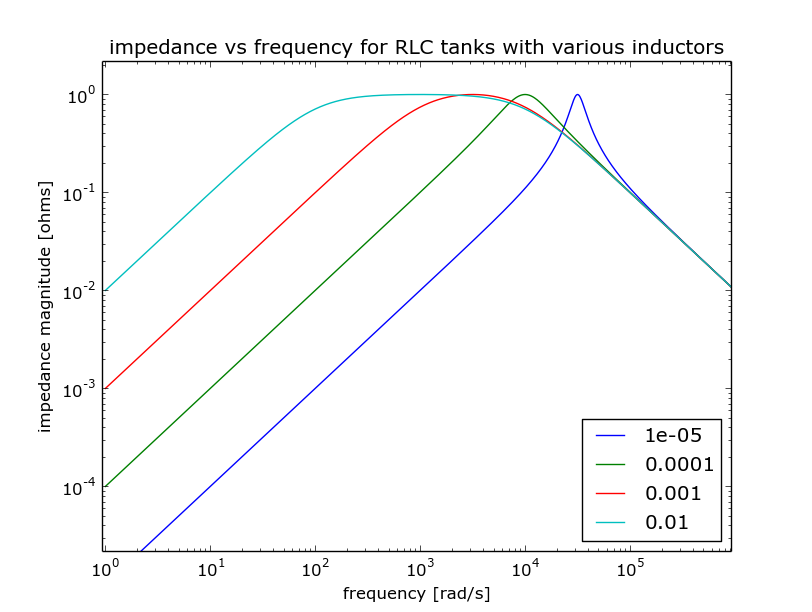
\includegraphics[width=0.35\textwidth]{inductors.png}
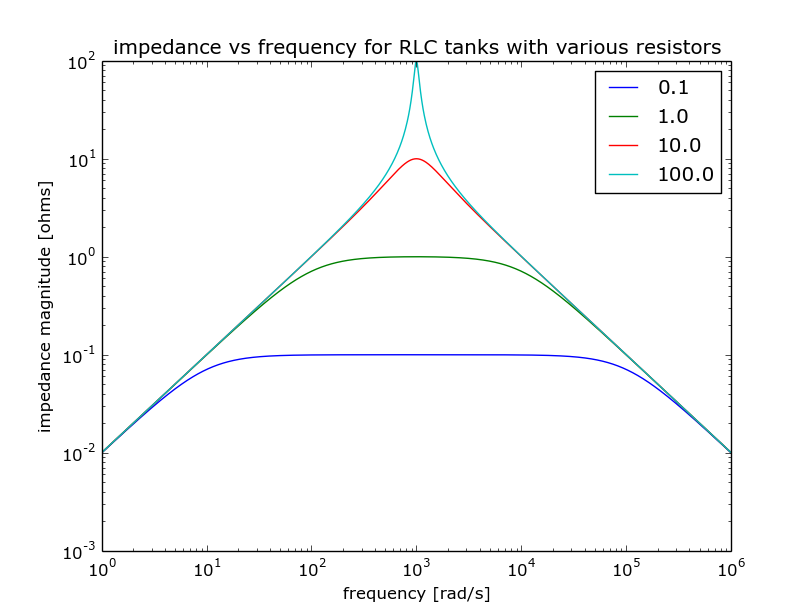
\includegraphics[width=0.35\textwidth]{resistors.png}
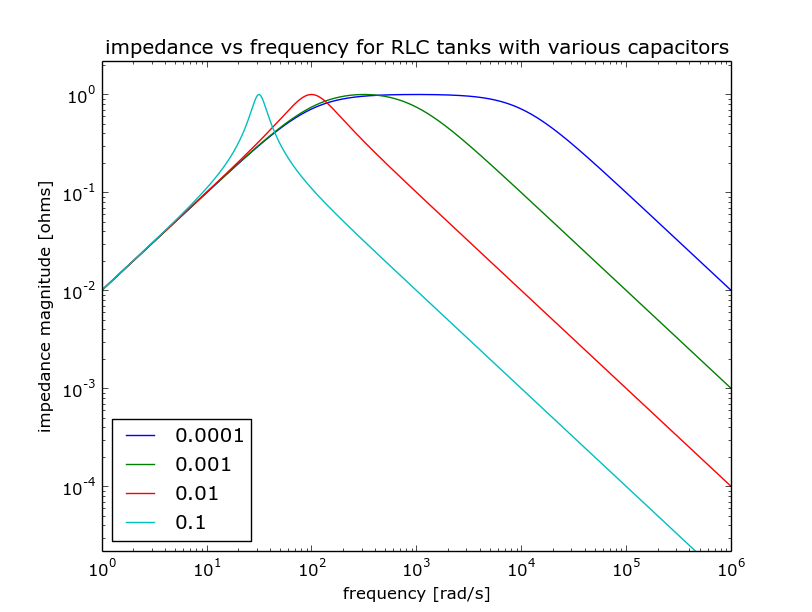
\includegraphics[width=0.35\textwidth]{capacitors.png}\\
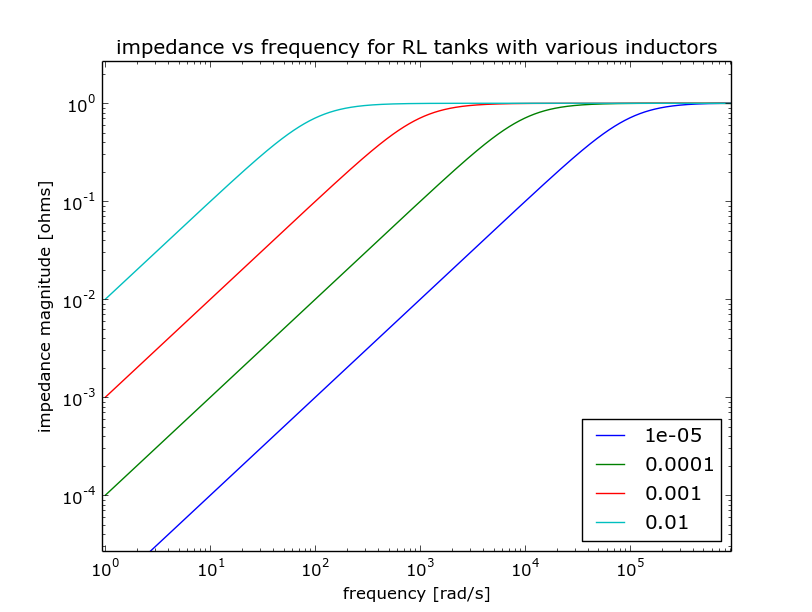
\includegraphics[width=0.35\textwidth]{rL.png}
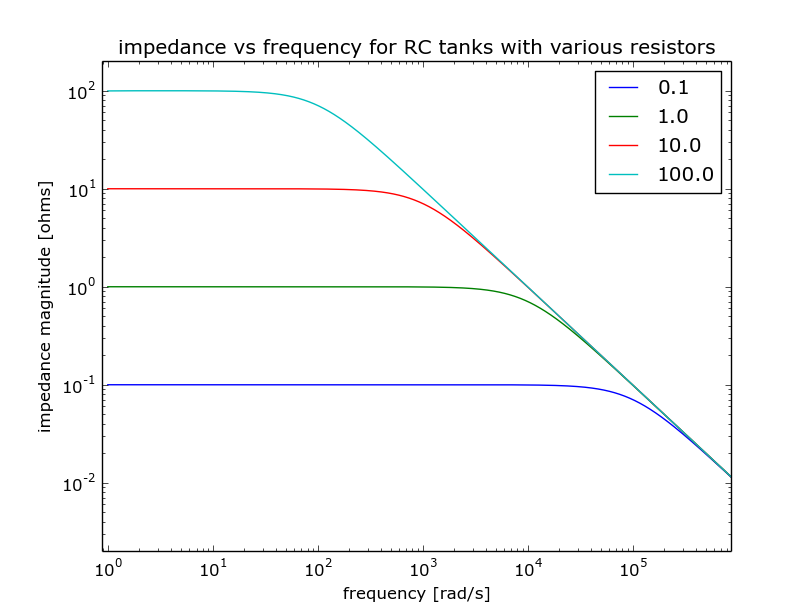
\includegraphics[width=0.35\textwidth]{Rc.png}
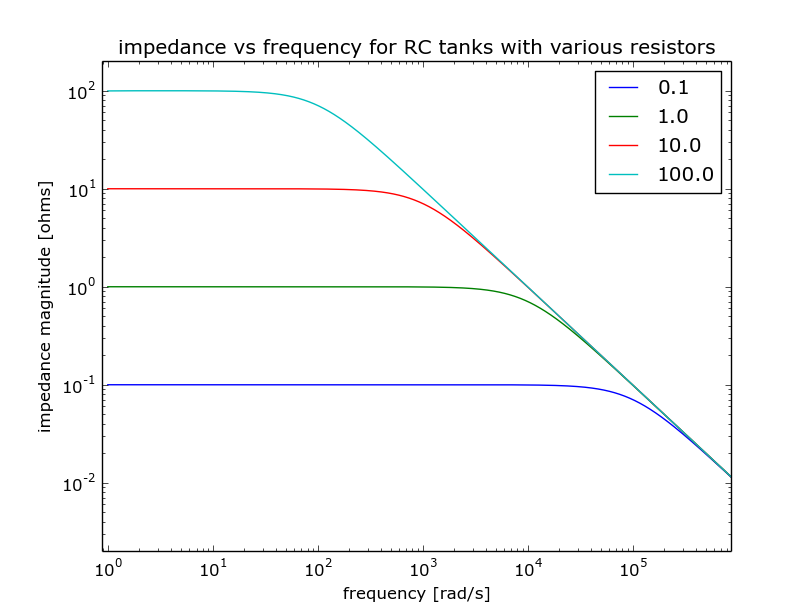
\includegraphics[width=0.35\textwidth]{rC.png}\\


If we look at the plots above, we can see that varying the resistance changes the maximum impedance over all frequencies, varying the inductance drops the asymptotic impedance at low frequencies, and varying the capacitance drops the asymptotic impedance at high frequencies.
We can imagine there are three regimes on the impedance vs frequency plot that divide the operation of an RLC tank into three elements:\\
When the slope is +1, the tank behaves like an inductor
$L=|Z|/(j\omega)$.
When the slope is -1, the tank behaves like a capacitor
$C=j\omega |Z|$.
When the slope is 0, the tank behaves like a resistor
$R=|Z|$.
This behavior can be exploited to reveal what elements are in parallel with one another.
First, sample at the highest possible driving frequency and a decade lower in frequency.
If the impedance increases by a decade, then there is a capacitor with capacitance $C=j\omega |Z|$.
Then, sample at the lowest reasonable driving frequency and a decade higher in frequency.
If the impedance increases by a decade, then there is an inductor with inductance $L=|Z|/(j\omega)$.
If there is an inductor and a capacitor, find the equivalent parallel resistance by sampling at $\omega=\sqrt{LC}^{-1}$.
If there is only a capacitor, find the equivalent parallel resistance by sampling at the lowest reasonable driving frequency.
If there is only an inductor, find the equivalent parallel resistance by sampling at the highest reasonable driving frequency.
If there is no capacitor and no inductor, sample mid-band.
An open circuit between two nodes will be indicated by an extremely high resistive reading and a low capacitance reading.

Diodes are indicated by asymmetric resistances.
For example, if $R_{12}=100\Omega$ and $R_{21}=1\Omega$, there is likely a diode between nodes 1 and 2.

\subsection{Software Test-bench}

A software test-bench was written to quickly iterate and test the circuit-sensing algorithm.
The test-bench uses NGspice, an open-source circuit simulator, to simulate a circuit and return only the data that would be accessible to the hardware test bench.
It includes a method to generate a random circuit with a specified number of nodes and types of circuit element, a method to insert probes, ground nodes, and voltage sources into an existing circuit, and a method to execute the simulation and format the results into a python-friendly output.
[I sincerely regret using python to implement this algorithm and intend to port the algorithm to julia or another, friendlier, language.]

Circuits are described by netlists (text descriptions of a circuit) where each line specifies a new branch in the network.
Each branch is composed of a circuit element (resistor, voltage source, etc.) with specified circuit parameter(s) (resistance, voltage, etc.), connected between a set of nodes.
Netlists are convenient here because they allow for insertion of circuit elelments, voltage sources, probes, and grounds with the addition of simple strings to a text file.

To write a random circuit netlist, the test-bench generates a random symmetric n-by-n matrix for each desired circuit element type, where n is the desired number of nodes in the circuit, excluding 'ground'.
The circuit elements explored in the scope of this thesis are resistors, capacitors, and inductors.
Each matrix is interpreted as a graph connecting the nodes in one dimension of the matrix to the nodes in the other dimension of the matrix.
The value at each location in the matrix is the circuit parameter for that particular element.
%----------------------Matrix -> Circuit -> Netlist Example---------------------
The matrix is used to generate a list of strings that are then inserted into a spice netlist.
At this point, the netlist only describes the random circuit generated and contains none of the 'machinery' required to reverse-engineer the circuit.

The circuit sensing algorithm conducts experiments on the circuit at hand and uses the data recorded to reverse-engineer the circuit.
These experiments are implemented by simulating the effect of adding voltage sources, grounding nodes, reading node voltages, and reading the current through the voltage sources.

Voltage sources are added by inserting a voltage source into the existing circuit netlist with an AC or a DC voltage.
Nodes are grounded by inserting a voltage source with zero DC voltage with respect to ground.
In the hardware test bench, nodes are grounded by a MOSFET connecting each rail to ground.
On the other hand, voltage sources are driven by a buffered DAC and multiplexed out to all of the nodes.
Since we have access to the voltage source, we can measure the current supplied by the buffered DAC and use that to gain information about the circuit in question.
This is a better idea as there are fewer current sensors required.


\subsection{PCB integration of Breadboard}

Tool design is an art.
There are many fields of study dedicated to the art of design, none of which I've spent much time exploring.
Despite this, I have developed my own sense for how tools should feel when they're in use.
The circuit-sensing breadboard should seem no different in both size and weight from a standard breadboard.
(I'm not saying that standard breadboards are perfect, but I am deciding not to spend time redesigning the breadboard)
To that end, I've decided that the best way to interface with an existing breadboard is to physically mount that breadboard on a printed circuit board.
I've developed a new technique for mounting a breadboard on a PCB.

A modern solderless breadboard is usually composed of three components - a plastic face, metal finger springs (rails), and a foam backing.
%---------------------DECONSTRUCTED BREADBOARD FIGURE---------------------------
The finger springs are designed to fit snugly in the plastic face, which provides structure for the entire board.
The foam backing keeps the finger springs from being pushed out the back of the plastic face.
A breadboard can be mounted to a PCB by removing the foam backing and surface mount soldering the finger springs to a PCB, then pressing the plastic face onto the mounted rails.

Initial tests of this technique involved small numbers of finger springs hand-soldered one-by-one to a PCB, using nail polish as soldermask.
%----------------------------1ST PROTOTYPE------------------------------------
The results of these tests were promising, but alignment proved to be an issue.
To mitigate this, a rail-holder was 3d-printed to losely hold each finger spring in precise alignment for PCB mounting.
%-----------------------RAIL HOLDER+GLUE AND PASTE----------------------------
Once all of the rails were inserted upside-down in the rail-holder, a dot of super glue between two dots of solderpaste were dispensed on each rail.
The rails were then adhered to the PCB by pressing the PCB upside-down onto the array of aligned rails, such that the rails lined up with pads on the PCB.
To aide with alignment during mounting, the rail-holder had four global alignment pegs that mated with four holes drilled into the PCB.
Finally the assembly was reflowed with hot air and the plastic faceplate was pressed on.
%-------------------UPSIDE DOWN PCB+SOLDERED RAILED+FINISHED------------------
%This process was successful and seems feasible for high-production runs, though I should probably talk to an expert on the subject.

%With a good PCB-Breadboard interface, a hardware test-bench was designed and fabricated.


\subsection{Hardware Test-bench}

The hardware test-bench is composed of a multiplexed network of voltage sensors, current sensors, signal generators, and a grounding network all orchestrated by a microcontroller.

In the hardware test bench, these voltage sources will be driven by a buffered DAC and multiplexed out to all of the nodes.
Since we have access to the voltage source, we can measure the current supplied by the buffered DAC and use that to gain information about the circuit in question.

In practice, designing a hardware test-bench that can perform comparably to the software test-bench is difficult.
The largest hurdle to taking high accuracy measurements is dynamic range.
Computers with 64-bit floating point numbers can easily handle six orders of magnitude while simulating circuits.
Designing an analog circuit that operates well over six orders of magnitude is no simple task.
(ie. a current sensor that operates over six orders of magnitude, a voltage sensor that operates over six orders of magnitude, an ADC that operates well over six orders of magnitude, etc.)


\subsubsection{Programming}

In order to handle the high datarates associated with capturing eight 1MSPS ADCs we use the Direct Memory Access (DMA) controller to asynchronously store samples.
Triggered by a timer interrupt, the DMA controller can store 8-bit wide GPIO port data.
Since the ADCs are serial output devices each additional ADC-sample-bit read will create an 8-bit wide piece of data, one bit for each ADC.
This data will have to be decoded later on to achieve high sample rates.

\subsubsection{Timers}

To clock the SPI ADCs we need a clock signal.
There are several timers to choose from on our microcontroller of choice, but we'll look at timers 2-5.

\subsubsection{STM32 stuff}

\subsubsection{Arduino stuff}
\begin{thebibliography}{1}
\end{thebibliography}
\end{document}
